\chapter{Tecnologie}
\label{chap:linguaggi-tecnologie}
%\footnote{\cite{site:agile-manifesto}} per citare

\section{Linguaggi}
\subsection{HTML}
\noindent \acrshort{html} (\textit{HyperText Markup Language}) è il linguaggio di marcatura standard utilizzato per strutturare i contenuti delle pagine web. Non si tratta di un linguaggio di programmazione, ma di uno strumento che consente di definire gli elementi presenti su una pagina (come titoli, testi, immagini, link, \glslink{formg}{form}) assegnando loro un significato semantico tramite l’uso di tag. \\
Introdotto nel 1991 da Tim Berners-Lee, \acrshort{html} si è evoluto nel tempo attraverso diverse versioni, fino a diventare uno standard globale supervisionato dal \textit{World Wide Web Consortium} (\acrshort{w3c}).\\
\\
La struttura di un file \acrshort{html} si basa su una serie di elementi, rappresentati attraverso tag, che permettono di definire la natura e la funzione dei contenuti all'interno di una pagina web. Ogni tag descrive una tipologia specifica di contenuto o un comportamento associato, contribuendo all'organizzazione semantica del documento. I tag sono delimitati da parentesi angolari (\texttt{< >}) e, nella maggior parte dei casi, sono utilizzati in coppie: un tag di apertura e uno di chiusura, quest’ultimo contraddistinto da una barra (\texttt{</tag>}). Alcuni elementi, tuttavia, non necessitano di chiusura e sono detti auto-chiudenti, come ad esempio \texttt{<img>} per l’inserimento di immagini, o \texttt{<br>} per i ritorni a capo. Questa struttura gerarchica e nidificata consente al \glslink{browserg}{browser} di interpretare correttamente i contenuti, garantendo coerenza tra presentazione e significato.\\
\\
La versione attuale, HTML5, è stata rilasciata in modo stabile nel 2014.\\
HTML5 rappresenta un’evoluzione del linguaggio di \glslink{markupg}{markup} con l’obiettivo di ridurre la dipendenza da \glslink{pluging}{plugin} esterni, introducendo nuove funzionalità native. Tra le principali novità vi sono gli elementi \texttt{<canvas>}, \texttt{<video>} e \texttt{<audio>}, nuovi tag semantici per strutturare i contenuti (come articoli, intestazioni, sezioni) e controlli avanzati per i \glslink{formg}{form} (email, \acrshort{url}, numeri, date, ricerca). 
\\Vengono inoltre introdotti strumenti per la memorizzazione locale dei dati sul client tramite \texttt{localStorage} e \texttt{sessionStorage}.

\begin{figure}[H]
    \centering
    
\includegraphics[width=0.25\textwidth]{img/html5.png}
    \caption[Logo HTML5]{Logo HTML5}
\end{figure}

\subsection{CSS}
\noindent \acrshort{css} (\textit{Cascading Style Sheets}) è un linguaggio utilizzato per definire la presentazione dei documenti \acrshort{html} e \acrshort{xml}. Introdotto nel 1996 da Håkon Wium Lie, consente di separare la struttura dei contenuti dalla loro formattazione, migliorando la chiarezza del codice e facilitandone la manutenzione.\\ 
I fogli di stile permettono di specificare, tramite regole composte da selettori, proprietà e valori, l’aspetto degli elementi \acrshort{html}: layout, colori, font, margini, spaziature, effetti visivi, animazioni e molto altro. Le regole di stile possono essere inline (tramite tag \texttt{<style>} o con attributi style) oppure riportate in file esterni .css riutilizzabili. La prima soluzione non mantiene però una netta separazione tra struttura e contenuto, non rispettando quindi le best-practice del settore.\\ 
L'attuale versione, CSS3, è modulare e introduce importanti funzionalità come \texttt{flexbox}, \texttt{grid}, media query per il responsive design, transizioni, trasformazioni e nuovi selettori.
\begin{figure}[H]
    \centering
    
\includegraphics[width=0.25\textwidth]{img/css3.png}
    \caption[Logo CSS3]{Logo CSS3}
\end{figure}

\subsection{Prism.js}
\noindent Prism.js è una libreria JavaScript leggera ed estensibile progettata per evidenziare la sintassi del codice sorgente in modo chiaro e leggibile, rispettando gli standard moderni del web. \\
Supporta un’ampia gamma di linguaggi di programmazione e di \glslink{markupg}{markup}, ed è facilmente personalizzabile tramite temi e \glslink{pluging}{plugin}. \\
Grazie alla sua efficienza e semplicità di integrazione, viene utilizzata in milioni di siti web per migliorare la leggibilità del codice, rendendolo più comprensibile sia a sviluppatori che a utenti. E’ disponibile in diverse varianti, sia per il white-mode che per il dark-mode.\\
Nella mia estensione, Prism.js è stato integrato per colorare il codice sorgente del \acrshort{dom}, facilitando l’analisi e la comprensione della struttura \acrshort{html}.

\subsection{JavaScript}
\noindent JavaScript è un linguaggio di programmazione dinamico, interpretato ed orientato agli oggetti, progettato originariamente per rendere le pagine web interattive.\\ 
È stato sviluppato nel 1995 da Brendan Eich per Netscape con il nome LiveScript, e successivamente rinominato in JavaScript per motivi di marketing, pur non avendo legami diretti con il linguaggio Java. La sua standardizzazione è gestita da \textit{ECMA International}, sotto il nome ECMAScript.\\
\\
Concepito per essere eseguito direttamente all’interno del \glslink{browserg}{browser}, JavaScript consente di scrivere \glslink{scriptg}{script} incorporati nel codice \acrshort{html}, eseguibili senza compilazione al momento del caricamento della pagina. Questi \glslink{scriptg}{script} permettono di manipolare il \acrshort{dom} (Document Object Model), reagire agli eventi dell’utente (come click, input da tastiera o movimenti del mouse), modificare dinamicamente il contenuto della pagina e gestire funzionalità come validazioni, messaggi, animazioni, e interazioni \glslink{asincronog}{asincrone}.\\
Oltre alla manipolazione di elementi visivi, JavaScript permette di sfruttare numerose \acrshort{api} messe a disposizione dal \glslink{browserg}{browser}, dalla gestione del mouse e del touch, alla manipolazione delle immagini, fino alla gestione locale dei dati attraverso meccanismi come il LocalStorage. Questa versatilità lo rende uno strumento fondamentale per lo sviluppo di applicazioni web moderne.\\
\\
JavaScript si è evoluto da semplice linguaggio \glslink{client-sideg}{client-side} a tecnologia completa e versatile, oggi utilizzabile anche su \glslink{serverg}{server} (ad esempio con \textit{Node.js}) e in ambienti esterni ai \glslink{browserg}{browser} grazie all’uso di diversi motori JavaScript i quali permettono l’esecuzione di codice \acrshort{js} con alte prestazioni, rendendo il linguaggio adatto anche a contesti \glslink{backendg}{backend}, applicazioni desktop e mobile.\\
Oggi JavaScript rappresenta uno dei tre pilastri fondamentali del web, insieme a \acrshort{html} e \acrshort{css}, ed è completamente integrato con essi. Esistono anche linguaggi alternativi (come TypeScript o CoffeeScript) che vengono compilati in JavaScript, offrendo funzionalità aggiuntive mantenendo la compatibilità con l’ambiente JavaScript standard.
\begin{figure}[H]
    \centering
    
\includegraphics[width=0.2\textwidth]{img/javascript.png}
    \caption[Logo JavaScript]{Logo JavaScript}
\end{figure}

\section{Tecnologie e strumenti}
\subsection{Chrome Extension}
\noindent Le estensioni di Chrome sono piccoli programmi software che consentono di arricchire e personalizzare il \glslink{browserg}{browser}, aggiungendo funzionalità aggiuntive o migliorando quelle già esistenti.\\
Grazie ad esse è possibile modificare l’interfaccia utente, automatizzare attività ripetitive, integrare servizi esterni e rendere più efficiente la navigazione sul web.\\ 
La distribuzione delle estensioni avviene principalmente tramite il \textit{Chrome Web Store}, ma durante le fasi di sviluppo è possibile installarle manualmente utilizzando la modalità sviluppatore disponibile nel \glslink{browserg}{browser}.

\subsubsection{Manifest V3}
\noindent Manifest V3 (\acrshort{mv3}) è la specifica più recente per la creazione di estensioni per Chrome e altri \glslink{browserg}{browser} basati su \textit{Chromium}. \\Rispetto alla precedente Manifest V2, l'ultima versione introduce diverse modifiche per migliorare la sicurezza, le prestazioni e la privacy delle estensioni.  \\
Questa nuova versione è una risposta alle criticità emerse con il Manifest V2, e introduce cambiamenti strutturali significativi nel modo in cui le estensioni interagiscono con il \glslink{browserg}{browser} e le pagine web.\\
E' importante notare che Manifest V3 non è retrocompatibile con le estensioni V2 senza modifiche sostanziali e che la versione è tuttora in evoluzione, poiché alcune funzionalità sono ancora in fase di implementazione.\\
Il file \texttt{manifest.json} in \acrshort{mv3} continua a rappresentare il cuore dell’estensione, definendo metadati fondamentali come nome, versione, permessi richiesti e \glslink{scriptg}{script} da eseguire. Tuttavia, rispetto a \acrshort{mv2}, \acrshort{mv3} impone restrizioni più rigide su quali \acrshort{api} possono essere utilizzate e introduce un modello di esecuzione più efficiente e sicuro.\\

\noindent Gli elementi principali di un’estensione basata su Manifest V3 sono:
\begin{itemize}
    \item \textbf{Manifest}: come nelle versioni precedenti, il file \texttt{manifest.json} contiene tutte le informazioni necessarie per il funzionamento dell’estensione, inclusi i permessi richiesti. 
    Tra i permessi più rilevanti vi sono: \begin{itemize}
        \item downloads: permette all’estensione di avviare e gestire download di file, ad esempio per salvare contenuti generati o analizzati;
        \item scripting: consente l’esecuzione di \glslink{scriptg}{script} personalizzati nelle pagine web, utile per analizzare o modificare il \acrshort{dom};
        \item activeTab: garantisce l’accesso temporaneo alla scheda attiva dopo un interazione dell’utente con l’estensione;
        \item tabs: fornisce informazioni sulle schede del \glslink{browserg}{browser} e permette di interagire con esse, come ottenere \acrshort{url} o titoli;
        \item storage: consente di memorizzare e recuperare dati locali, ad esempio impostazioni o risultati di analisi.
    \end{itemize}
    \item \textbf{Service Worker}: in Manifest V3, i tradizionali background \glslink{scriptg}{script} sono sostituiti da service worker. Questi sono \glslink{scriptg}{script} che vengono eseguiti in background ma solo quando necessario, rispondendo a eventi come le richieste di rete o azioni dell’utente. A differenza dei background \glslink{scriptg}{script} di \acrshort{mv2}, i service worker non sono persistenti e vengono sospesi quando inattivi, riducendo così l’utilizzo di risorse e migliorando le prestazioni complessive. I service worker non possono accedere direttamente al \acrshort{dom} delle pagine, ma comunicano con i content \glslink{scriptg}{script} tramite messaggi.
    \item \textbf{Content Script}: vengono iniettati direttamente nelle pagine web e possono interagire con il \acrshort{dom}. In \acrshort{mv3}, anche i content \glslink{scriptg}{script} sono soggetti a restrizioni più severe per evitare conflitti con il contenuto della pagina e migliorare la sicurezza.
\end{itemize}
\vspace{0.5cm}
\noindent Il Manifest V3 introduce modifiche significative nell’ecosistema delle estensioni per \glslink{browserg}{browser}, con effetti sia positivi sia problematici.\\
\\
\textbf{Aspetti positivi}\\
Tra i vantaggi più evidenti vi è il blocco del codice remoto, che impedisce alle estensioni di scaricare ed eseguire codice non verificato dopo l’installazione. Questa misura contribuisce a ridurre alcuni rischi di sicurezza, proteggendo gli utenti da esecuzioni di codice potenzialmente dannoso.\\
\\
\textbf{Aspetti critici}\\
Il nuovo standard non elimina completamente i rischi: le \acrshort{api} continuano a consentire la raccolta di dati sensibili (come la cronologia di navigazione) lasciando alcune vulnerabilità inalterate. \\Dal punto di vista dello sviluppo, \acrshort{mv3} comporta limitazioni importanti: l'\acrshort{api} \texttt{webRequest}, utilizzata per modificare dinamicamente le richieste di rete, è stata sostituita da \texttt{declarativeNetRequest}, più rigida e meno flessibile, riducendo le possibilità di innovazione. \\Inoltre, le pagine background persistenti vengono sostituite dai service worker, che presentano vincoli sulle \acrshort{api} disponibili e problemi di compatibilità con funzioni avanzate ( come \glslink{websocketg}{WebSockets}, \glslink{webassemblyg}{WebAssembly} o la localizzazione delle estensioni). 
\\La migrazione a \acrshort{mv3} si è dimostrata complessa e molte funzionalità di estensioni pre-esistenti rischiano di rompersi o di subire un peggioramento delle prestazioni. Infine, il processo decisionale di Google è stato percepito come scarsamente collaborativo, poiché l’implementazione del nuovo standard è stata imposta senza un reale dialogo con la comunità degli sviluppatori.\\
\\
In sintesi, sebbene il blocco del codice remoto rappresenti un progresso in termini di sicurezza, Manifest V3 introduce restrizioni che limitano innovazione, privacy e performance, portando l’\textit{Electronic Frontier Foundation} a definirlo un atto ostile verso gli utenti, frutto di una posizione dominante di Google nell’ecosistema delle estensioni web.

\subsection{Ollama}
\noindent Ollama è una piattaforma che consente di eseguire localmente modelli di \glslink{iag}{intelligenza artificiale} avanzati, sviluppati in collaborazione con OpenAI e altri partner, mantenendo alte prestazioni anche senza l’uso del \glslink{cloud-computingg}{cloud computing}. 
Oltre ai modelli gpt-oss-20B e gpt-oss-120B, progettati rispettivamente per scenari a bassa \glslink{latenzag}{latenza} o per applicazioni generali ad alto livello di ragionamento, Ollama supporta numerosi altri modelli \glslink{open-weightg}{open weight}, tra cui Mistral (utilizzato solo all’inizio a causa delle ridotte capacità del mio pc personale), Llama 3.1:8B e Llama 3.2:3B, che ho utilizzato nel mio progetto. Nella tabella sottostante ~\ref{tab:modelli-ollama} vengono messi a confronto i vari modelli di Ollama utilizzati nei test dell'estensione \textit{SviluppAbile}.\\ 

\begin{longtable}[c]{|C{3cm}||C{3.5cm}|C{3.5cm}|C{3.5cm}|}
\caption{Confronto modelli Ollama utilizzati}
\label{tab:modelli-ollama}\\
\hline
\textbf{Versione} & \textbf{Llama 3.1:8b} & \textbf{Llama 3.2:3b} & \textbf{Mistral}\\
\hline
\endfirsthead
\multicolumn{3}{c}%
{{\bfseries Table \thetable\ -- continua dalla pagina precedente}} \\
\hline
\textbf{Versione: } & \textbf{Llama 3.1:8b} & \textbf{Llama 3.2:3b} & \textbf{Mistral}\\
\hline
\endhead
\hline
\multicolumn{3}{r}{{ -- continua nella pagina successiva}} \\
\endfoot
\hline
\endlastfoot
\textbf{Ragionamento complesso} & Molto elevato, ottimo su coding, Q\&A, compiti multilingue complessi & Buono ma inferiore ai modelli più grandi, migliore per compiti rapidi & Limitato rispetto a Llama 8b, pensato per compiti specifici\\
\hline
\textbf{Comprensione linguistica} & Alta precisione e coerenza, anche in testi lunghi & Discreta, ma può generare errori grammaticali o essere meno coerente in testi lunghi & Buona solo in testi brevi e semplici \\
\hline
\textbf{Conoscenza generale} & Ampia copertura di argomenti & Più ridotta per via del minor numero di parametri & Limitata\\
\hline
\textbf{Velocità di risposta} & Più lenta su hardware modesto & Rapida con HW adeguato & Molto rapida\\
\hline
\textbf{Requisiti hardware} & Almeno 8 GB RAM + richiede \acrshort{gpu} di fascia media/alta & Almeno 4 GB RAM & Almeno 2 GB RAM \\
\hline
\end{longtable}

\noindent La piattaforma integra funzionalità avanzate (function calling, navigazione web integrata, esecuzione di codice Python, output strutturati), accesso completo al processo di ragionamento del modello, regolazione dello sforzo computazionale e possibilità di fine-tuning per personalizzare le prestazioni. 
Grazie al supporto nativo per la \glslink{quantizzazioneg}{quantizzazione} in formato MXFP4, Ollama riesce a ridurre drasticamente il consumo di memoria, permettendo l’esecuzione di modelli molto grandi anche su sistemi con risorse limitate. 
La licenza Apache 2.0 garantisce libertà di utilizzo e personalizzazione, mentre l’ottimizzazione per \acrshort{gpu} NVIDIA GeForce RTX e RTX PRO assicura alte prestazioni in locale.
.
\begin{figure}[H]
    \centering
    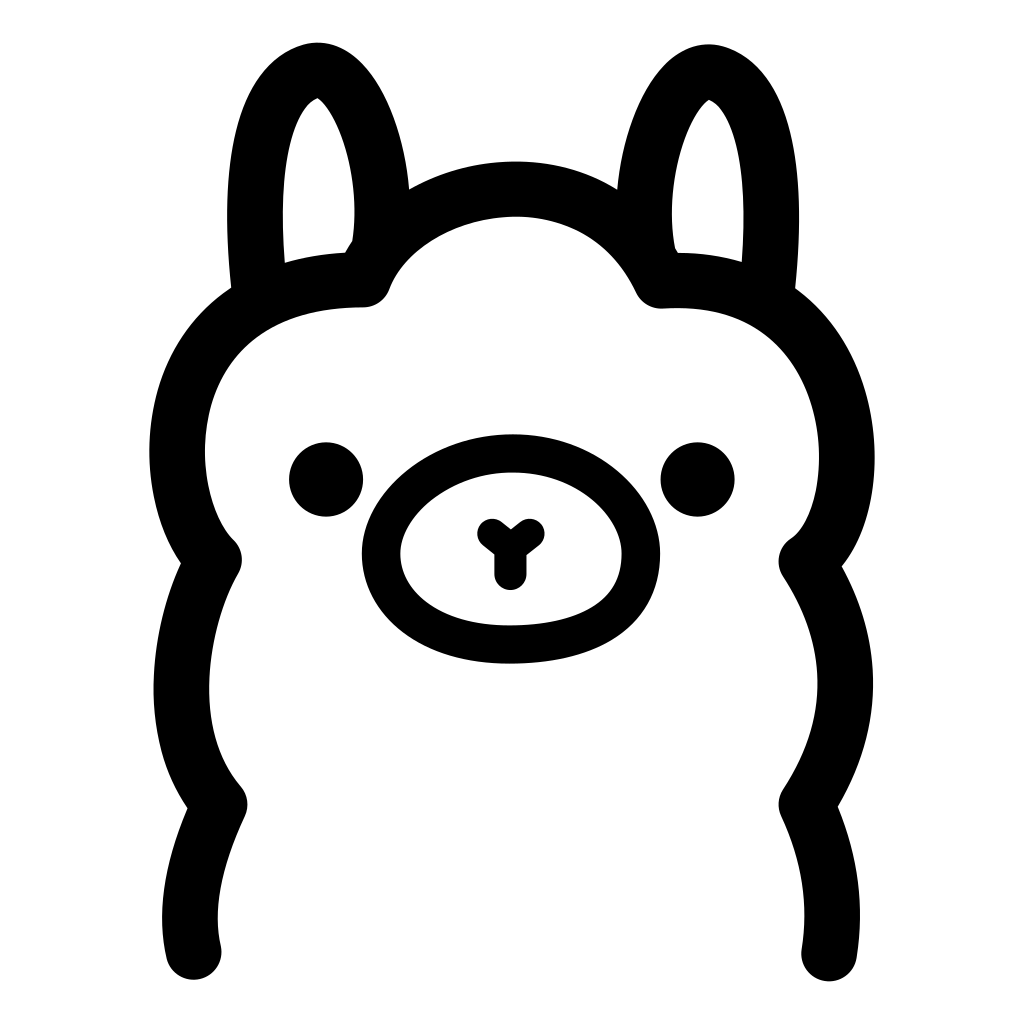
\includegraphics[width=0.2\textwidth]{img/ollama.png}
    \caption[Logo Ollama]{Logo Ollama}
\end{figure}


\subsection{GitHub}
\noindent GitHub è una piattaforma di hosting basata su \glslink{gitg}{Git}, il sistema di controllo di versione distribuito ideato da Linus Torvalds. Lanciata nel 2008, GitHub si è affermata come uno degli strumenti principali per la collaborazione nello sviluppo software, consentendo a sviluppatori di tutto il mondo di condividere, modificare e mantenere progetti in modo coordinato. \\La piattaforma offre funzionalità avanzate per il versionamento del codice, la gestione dei rami (branching), il tracciamento delle modifiche e la revisione collaborativa tramite pull request. \\Oltre a essere uno strumento tecnico, GitHub ha favorito la nascita di una vera e propria comunità \glslink{open-sourceg}{open source}, nella quale il codice è accessibile, riutilizzabile e migliorabile da chiunque.
\begin{figure}[H]
    \centering
    
\includegraphics[width=0.2\textwidth]{img/github.png}
    \caption[Logo GitHub]{Logo GitHub}
\end{figure}

\subsection{VSCode}
\noindent Visual Studio Code, conosciuto semplicemente come VSCode, è un editor di codice sorgente sviluppato da Microsoft e distribuito gratuitamente. Introdotto nel 2015, ha rapidamente conquistato una posizione di rilievo tra gli strumenti preferiti dagli sviluppatori grazie alla sua combinazione di leggerezza, flessibilità e ricchezza di funzionalità. \\Compatibile con i principali sistemi operativi (Windows, macOS e Linux), VSCode supporta evidenziazione della sintassi per numerosi linguaggi, suggerimenti intelligenti e completamento automatico del codice, strumenti di \glslink{debuggingg}{debugging} integrati e gestione del controllo di versione tramite \glslink{gitg}{Git}. \\Inoltre, grazie a un vasto marketplace di estensioni, può essere facilmente personalizzato per adattarsi a diversi flussi di lavoro e tecnologie, rendendolo un ambiente di sviluppo versatile e ampiamente diffuso.
\begin{figure}[H]
    \centering
    
\includegraphics[width=0.25\textwidth]{img/vscode.jpg}
    \caption[Logo VSCode]{Logo VSCode}
\end{figure}

\subsection{Total Validator}
\noindent ...
\begin{figure}[H]
    \centering
    
\includegraphics[width=0.2\textwidth]{img/totalvalidator.png}
    \caption[Logo Total Validator]{Logo Total Validator}
\end{figure}
\newpage